\documentclass[conference]{IEEEtran}
\IEEEoverridecommandlockouts
\usepackage{cite}
\usepackage{amsmath,amssymb,amsfonts}
\usepackage{algorithm}
\usepackage{algorithmic}
\usepackage{graphicx}
\usepackage{textcomp}
\usepackage{xcolor}
\usepackage{booktabs}
\usepackage{multirow}
\usepackage{array}
\usepackage{url}
\usepackage{enumitem}
\setlist{leftmargin=*, labelindent=\parindent, itemsep=1pt, topsep=2pt}
\usepackage{tikz}
\usetikzlibrary{shapes.geometric,arrows.meta,positioning,calc}
\usepackage{pgfplots}
\pgfplotsset{compat=1.17}

\begin{document}

\title{FinGraph AI: A Temporal Knowledge Graph and\\ Hybrid GraphRAG Framework for Multi-Hop\\ Financial Question Answering}

\author{
\IEEEauthorblockN{Dhruv VM}
\IEEEauthorblockA{\textit{Dept. of CSE (AIML)}\\
\textit{Dayananda Sagar University}\\
Bengaluru, India\\
eng24am0165@dsu.edu.in}
\and
\IEEEauthorblockN{Mohammed Talha}
\IEEEauthorblockA{\textit{Dept. of CSE (AIML)}\\
\textit{Dayananda Sagar University}\\
Bengaluru, India\\
eng24am0051@dsu.edu.in}
\and
\IEEEauthorblockN{Ranjith Gowda}
\IEEEauthorblockA{\textit{Dept. of CSE (AIML)}\\
\textit{Dayananda Sagar University}\\
Bengaluru, India\\
eng24am0072@dsu.edu.in}
\and
\IEEEauthorblockN{Tejas Yadav D}
\IEEEauthorblockA{\textit{Dept. of CSE (AIML)}\\
\textit{Dayananda Sagar University}\\
Bengaluru, India\\
eng24am0305@dsu.edu.in}
}

\maketitle

\begin{abstract}
Answering financial questions from regulatory filings requires reasoning across several entities and documents while respecting when each fact became public. Conventional Retrieval-Augmented Generation (RAG) treats documents as timeless, can let one dominant company crowd out evidence for another in comparative questions, and tends to answer even when the evidence is insufficient. This paper presents FinGraph AI, a temporal knowledge graph and hybrid GraphRAG framework for multi-hop question answering over U.S. SEC filings. The framework combines structure-aware chunking with filing-availability timestamps, a temporal knowledge graph built from extracted entities and relations, dense vector retrieval, and breadth-first graph traversal. Candidates are merged with Entity-Balanced Reciprocal Rank Fusion (EB-RRF), which reserves evidence slots for every company named in a query. An adaptive hop-depth gate, regulatory entity linking and an evidence-sufficiency check then decide whether to generate a cited answer or return a controlled refusal. On a corpus of 99 filings from 10 companies (8,181 chunks; 10,054 graph nodes; 9,822 edges) and a verified 64-question benchmark, the full configuration made the correct answer-or-refuse decision on 59 of 64 questions (92.19\%), up from 55 of 64 (85.94\%) for the base configuration. It refused all 14 unanswerable questions and retrieved no evidence published after a query's reference date. The gains were concentrated in multi-hop and cross-document questions. A post-hoc audit, however, found that only 34 of the 45 answers were fully supported, and answerable Token F1 remained modest at 0.3229. Decision-level safety therefore outpaces answer completeness, and we report both.
\end{abstract}

\begin{IEEEkeywords}
Financial Question Answering, Temporal Knowledge Graphs, GraphRAG, Hybrid Retrieval, Reciprocal Rank Fusion, Multi-Hop Reasoning, Evidence Grounding, Controlled Refusal, SEC Filings.
\end{IEEEkeywords}

%=====================================================================
\section{Introduction}
%=====================================================================
Financial question answering involves more than locating a sentence in a corporate disclosure. An analyst asking which regulator challenged an acquisition, or how two companies describe the same competitive market, must connect facts that sit in different filings, link them through named entities, and use only information that was public at the time of interest. Large Language Models (LLMs) produce fluent answers to such questions but may state facts the sources do not support. Retrieval-Augmented Generation (RAG) reduces this risk by conditioning generation on retrieved text, and it has been applied to financial trend analysis~\cite{ertugrul2026rag}. Knowledge-graph integration with transformer models has been studied for financial representation and analysis~\cite{yahathugoda2026kgatfin,yarlagadda2026kg}. Dynamic knowledge graphs have been used for evolving business insights~\cite{jain2025dynamic}, and graph-based reasoning has been proposed to strengthen LLMs~\cite{chai2026graphllm}.

Three practical problems remain when these ideas are applied to SEC filings:
\begin{enumerate}
\item \textit{Temporal leakage.} A retriever that ignores filing dates can answer a question ``as of'' a past date using a disclosure filed later. This is the retrieval analogue of look-ahead bias in financial modelling.
\item \textit{Entity starvation in comparative and multi-hop queries.} Standard Reciprocal Rank Fusion (RRF) can fill every evidence slot with chunks about the company that matches the query most strongly, leaving none for the second company the question requires.
\item \textit{Over-answering.} When evidence is missing, a generator that always answers will produce unsupported statements. A financial system should recognise insufficient evidence and abstain.
\end{enumerate}

This paper presents FinGraph AI, a temporal knowledge graph and hybrid GraphRAG framework that targets these problems. Its contributions are:
\begin{itemize}
\item A pipeline that attaches a filing-availability timestamp to every chunk and graph edge and enforces a point-in-time eligibility constraint at retrieval and citation time.
\item Entity-Balanced Reciprocal Rank Fusion (EB-RRF), which reserves a minimum number of verified evidence slots for each required entity before filling the remainder by global rank.
\item An adaptive hop-depth gate and regulatory/jurisdictional entity linking that let directly stated relationships satisfy relational queries while still requiring complete chains for explicitly compound questions.
\item An evaluation on a verified 64-question benchmark that reports answer and refusal behaviour separately, with a component ablation, a per-category breakdown and a post-hoc answer audit.
\end{itemize}
The overall architecture is shown in Fig.~\ref{fig:arch}.

\begin{figure}[t]
\centering
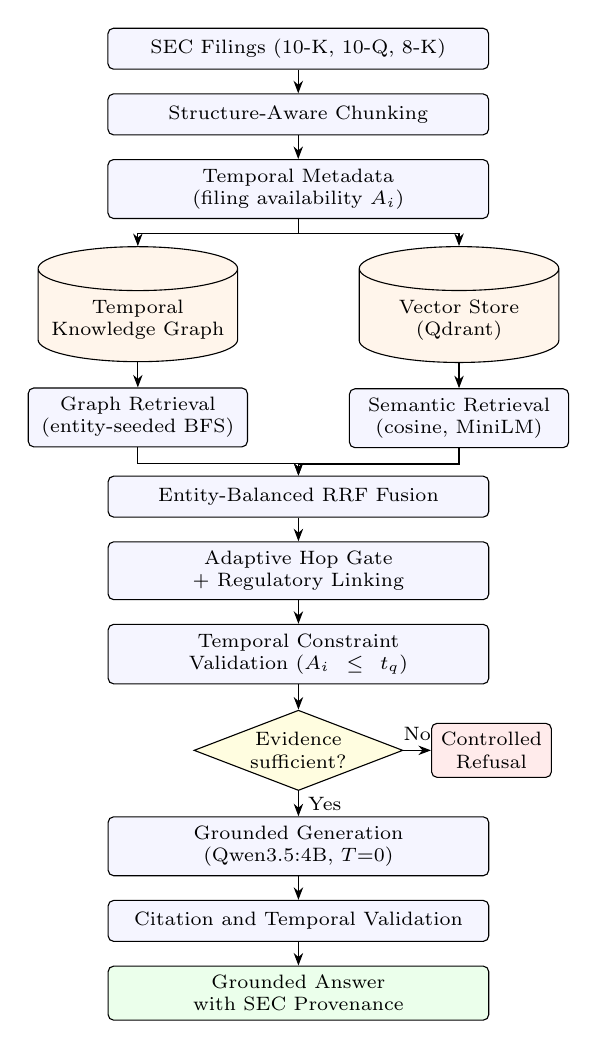
\begin{tikzpicture}[
  font=\scriptsize,
  box/.style={draw, rounded corners=2pt, align=center, minimum height=0.52cm, text width=#1, fill=blue!4},
  box/.default=4.6cm,
  store/.style={draw, cylinder, shape border rotate=90, aspect=0.22, align=center, minimum height=0.75cm, text width=2.3cm, fill=orange!8},
  dec/.style={draw, diamond, aspect=2.6, align=center, inner sep=1pt, fill=yellow!12},
  term/.style={draw, rounded corners=2pt, align=center, minimum height=0.52cm, fill=green!8},
  arr/.style={-{Stealth[length=1.6mm]}, thin},
  node distance=0.30cm
]
\node[box] (sec) {SEC Filings (10-K, 10-Q, 8-K)};
\node[box, below=of sec] (chunk) {Structure-Aware Chunking};
\node[box, below=of chunk] (meta) {Temporal Metadata (filing availability $A_i$)};
\node[store, below left=0.42cm and -1.25cm of meta] (kg) {Temporal\\Knowledge Graph};
\node[store, below right=0.42cm and -1.25cm of meta] (vdb) {Vector Store\\(Qdrant)};
\node[box=2.55cm, below=0.32cm of kg] (gr) {Graph Retrieval\\(entity-seeded BFS)};
\node[box=2.55cm, below=0.32cm of vdb] (vr) {Semantic Retrieval\\(cosine, MiniLM)};
\node[box] at ($(gr.south)!0.5!(vr.south)+(0,-0.62)$) (fuse) {Entity-Balanced RRF Fusion};
\node[box, below=of fuse] (hop) {Adaptive Hop Gate + Regulatory Linking};
\node[box, below=of hop] (tv) {Temporal Constraint Validation ($A_i \le t_q$)};
\node[dec, below=0.32cm of tv] (suf) {Evidence\\sufficient?};
\node[term, right=0.35cm of suf, fill=red!8] (ref) {Controlled\\Refusal};
\node[box, below=0.32cm of suf] (gen) {Grounded Generation (Qwen3.5:4B, $T{=}0$)};
\node[box, below=of gen] (cv) {Citation and Temporal Validation};
\node[term, text width=4.6cm, below=of cv] (out) {Grounded Answer with SEC Provenance};
\draw[arr] (sec) -- (chunk);
\draw[arr] (chunk) -- (meta);
\draw[arr] (meta.south) -- ++(0,-0.18) -| (kg.north);
\draw[arr] (meta.south) -- ++(0,-0.18) -| (vdb.north);
\draw[arr] (kg) -- (gr);
\draw[arr] (vdb) -- (vr);
\draw[arr] (gr.south) -- ++(0,-0.2) -| (fuse.north);
\draw[arr] (vr.south) -- ++(0,-0.2) -| (fuse.north);
\draw[arr] (fuse) -- (hop);
\draw[arr] (hop) -- (tv);
\draw[arr] (tv) -- (suf);
\draw[arr] (suf) -- node[above]{No} (ref);
\draw[arr] (suf) -- node[right]{Yes} (gen);
\draw[arr] (gen) -- (cv);
\draw[arr] (cv) -- (out);
\end{tikzpicture}
\caption{Overall architecture of the proposed FinGraph AI framework.}
\label{fig:arch}
\end{figure}

%=====================================================================
\section{Literature Review}
%=====================================================================
\subsection{Financial Question Answering, RAG and NLP}
Retrieval-Augmented Generation (RAG) has been applied to financial analysis: Ertu\u{g}rul et al.~\cite{ertugrul2026rag} built a RAG-based trend-analysis system for Borsa Istanbul indices. Van et al.~\cite{van2026llmstock} combined news sentiment and technical indicators for stock prediction, and Yang et al.~\cite{yang2025timerag} applied retrieval augmentation to time-series forecasting. Other work has studied earnings-call sentiment~\cite{icocics2025earnings} and representation bias in financial language models~\cite{sabuncuoglu2025bias}. These systems show the value of retrieval and language models in finance~\cite{ertugrul2026rag,van2026llmstock,yang2025timerag,icocics2025earnings,sabuncuoglu2025bias}, but they target trend analysis~\cite{ertugrul2026rag}, price and volatility prediction~\cite{van2026llmstock}, forecasting~\cite{yang2025timerag} or sentiment analysis~\cite{icocics2025earnings,sabuncuoglu2025bias} rather than cross-filing, multi-hop question answering with explicit refusal.

\subsection{Knowledge Graphs and Graph-Based Retrieval}
Knowledge graphs represent entities and typed relations explicitly, which makes multi-step connections retrievable~\cite{yarlagadda2026kg,chai2026graphllm}. KGATFin~\cite{yahathugoda2026kgatfin} augments transformers with knowledge-graph information for financial analytics. Yarlagadda~\cite{yarlagadda2026kg} combined knowledge-graph embeddings with transformers for financial document search, and Jain et al.~\cite{jain2025dynamic} used dynamic graphs and graph neural networks for business insights. GraphLLM~\cite{chai2026graphllm} improves graph reasoning in LLMs. These approaches~\cite{yahathugoda2026kgatfin,yarlagadda2026kg,jain2025dynamic,chai2026graphllm} focus on representation, sentiment, prediction or reasoning ability. Apart from the evolving graphs of~\cite{jain2025dynamic}, they treat edges as static facts, and none attaches the time at which each relation became publicly known.

\subsection{Temporal and Agentic Retrieval}
Temporal validity is central in finance because a disclosure can only inform decisions after it is published, and time-aware retrieval~\cite{yang2025timerag} and real-time financial decision systems~\cite{kamlakshya2025agentic} both depend on using information in the right time order. Using later information to explain an earlier state introduces look-ahead bias, which makes historical analysis unreliable. TimeRAG~\cite{yang2025timerag} brings retrieval to temporal forecasting, and Kamlakshya~\cite{kamlakshya2025agentic} proposed an agentic, multi-agent RAG framework with Model Context Protocol integration for real-time financial decisions. Neither~\cite{yang2025timerag,kamlakshya2025agentic} enforces point-in-time eligibility on evidence drawn from a graph and a vector index at the same time.

\subsection{Research Gap and Motivation}
Table~\ref{tab:lit} summarises the reviewed work~\cite{ertugrul2026rag,yahathugoda2026kgatfin,yarlagadda2026kg,jain2025dynamic,chai2026graphllm,van2026llmstock,yang2025timerag,icocics2025earnings,sabuncuoglu2025bias,kamlakshya2025agentic}. Existing approaches address financial RAG~\cite{ertugrul2026rag,kamlakshya2025agentic}, knowledge-graph construction~\cite{yahathugoda2026kgatfin,yarlagadda2026kg,jain2025dynamic} or graph reasoning~\cite{chai2026graphllm} in isolation. They do not jointly provide (i) point-in-time evidence eligibility, (ii) balanced evidence coverage for every entity a query names, (iii) relational retrieval over typed edges, and (iv) a decision to abstain when support is insufficient. FinGraph AI combines these four properties in a single pipeline and evaluates them on answer and refusal behaviour separately.

\begin{table*}[t]
\caption{Comparative Analysis of Existing Financial Research}
\label{tab:lit}
\centering
\footnotesize
\begin{tabular}{p{0.6cm}p{3.0cm}p{3.4cm}p{4.4cm}p{4.6cm}}
\toprule
\textbf{Ref.} & \textbf{Model Type} & \textbf{Data Characteristics} & \textbf{Key Strength} & \textbf{Key Limitation}\\
\midrule
\cite{ertugrul2026rag} & RAG, FAISS, intent classification & Borsa Istanbul indices and documents & Applies retrieval-based generation to financial trend analysis & Targets trend analysis rather than multi-hop QA\\
\cite{yahathugoda2026kgatfin} & BERT, KG embeddings, attention fusion & Financial text and ontologies & Injects domain knowledge into transformer-based sentiment analysis & Sentiment classification, not temporal QA\\
\cite{yarlagadda2026kg} & Transformer, KG embeddings & Structured and unstructured financial documents & Combines semantic representations with graph reasoning & Temporal validation left for future work\\
\cite{jain2025dynamic} & NLP, GNN, dynamic KG & Evolving business and financial data & Models changing business relationships & Predictive insights, not evidence-grounded QA\\
\cite{chai2026graphllm} & GraphLLM & Graph-structured data & Improves graph reasoning in LLMs & No temporal financial document retrieval\\
\cite{van2026llmstock} & Whisper, BART, FinGPT, multimodal & News sentiment and technical indicators & Fuses text and quantitative signals & Stock prediction, not multi-hop retrieval\\
\cite{yang2025timerag} & TimeRAG & Time-series data & Retrieval-based information integration for forecasting & Forecasting, not knowledge-graph QA\\
\cite{icocics2025earnings} & Whisper, BART, FinGPT & Earnings-call recordings and transcripts & Transcription, summarisation and sentiment & Earnings-call sentiment, not cross-document QA\\
\cite{sabuncuoglu2025bias} & LLMs, bias analysis & Financial sentiment data & Identifies representation bias & Bias analysis, not retrieval or reasoning\\
\cite{kamlakshya2025agentic} & Agentic RAG, multi-agent, MCP & Real-time financial information & Agent-based financial information processing & No temporal knowledge-graph QA\\
\bottomrule
\end{tabular}
\end{table*}

%=====================================================================
\section{Methodology}
%=====================================================================
\subsection{Problem Formulation}
Let $\mathcal{C}=\{c_1,\dots,c_N\}$ be the set of chunks derived from the filings, and let $G=(V,E,T)$ be the temporal knowledge graph. A query consists of a natural-language question $q$, an optional reference time $t_q$, and a set of required entities $\mathcal{E}_q$ identified in $q$. The system must either (i) select an evidence set $\mathcal{S}\subseteq\mathcal{C}\cup E$ in which every item was public at $t_q$, and generate an answer supported only by $\mathcal{S}$ with citations, or (ii) return a controlled refusal when $\mathcal{S}$ does not support an answer.

\subsection{SEC Data Collection and Preprocessing}
The corpus contains 99 filings retrieved from the SEC EDGAR system for ten publicly listed companies: Apple, Microsoft, NVIDIA, Alphabet, Amazon, Meta, Tesla, JPMorgan Chase, Johnson \& Johnson and ExxonMobil. It includes annual reports (Form 10-K), quarterly reports (Form 10-Q) and current reports (Form 8-K), with reporting periods from March 2025 to September 2026. Each filing is converted into normalised text that preserves section headings, paragraph boundaries and filing metadata, including the accession number and acceptance date.

\subsection{Structure-Aware Chunking and Temporal Metadata}
Rather than fixed-length splitting, filings are segmented along section and paragraph boundaries and paragraphs are merged up to a 1,800-character limit. Paragraphs that exceed the limit are split into deterministic windows with a 250-character overlap. Each chunk is represented as
\begin{equation}
C_i = (X_i, D_i, P_i, A_i, S_i)
\end{equation}
where $X_i$ is the text, $D_i$ the document metadata, $P_i$ the provenance (issuer and accession), $A_i$ the filing-availability timestamp and $S_i$ the source section. A chunk is temporally eligible for a query with reference time $t_q$ only if
\begin{equation}
A_i \le t_q .
\label{eq:elig}
\end{equation}
This uses the date the information became public, not the fiscal period it describes, so a 10-K for a year ending in December is unavailable until it is filed. Preprocessing produced 8,181 chunks.

\subsection{Temporal Knowledge Graph Construction}
Entities (companies, executives, products, business segments, suppliers, subsidiaries and regulators) and typed relations (e.g., \textsc{acquired}, \textsc{competes\_with}, \textsc{depends\_on}, \textsc{manufactures}) are extracted from each chunk with schema-constrained prompts and resolved to canonical identifiers. The graph is
\begin{equation}
G = (V, E, T), \qquad e_{ij} = (v_i, r_{ij}, v_j, \tau_{ij})
\end{equation}
where $v_i, v_j \in V$ are entities, $r_{ij}$ is the relation type, and $\tau_{ij}$ stores the event time and availability time of the supporting disclosure. Every edge keeps a pointer to its source chunk, so graph evidence can be cited to a filing. A $k$-hop path is
\begin{equation}
P_k = (v_0, r_1, v_1, \dots, r_k, v_k).
\end{equation}
The constructed graph contains 10,054 nodes and 9,822 edges.

\subsection{Hybrid Graph and Vector Retrieval}
\textit{Semantic retrieval.} Queries and chunks are embedded with the 384-dimensional all-MiniLM-L6-v2 sentence-embedding model and stored in Qdrant. Candidates are ranked by cosine similarity
\begin{equation}
\mathrm{Sim}(\mathbf{q},\mathbf{d}_i) = \frac{\mathbf{q}\cdot\mathbf{d}_i}{\|\mathbf{q}\|\,\|\mathbf{d}_i\|}.
\end{equation}

\textit{Graph retrieval.} Entities linked in the query seed a breadth-first search over $G$ (up to two hops by default, at most three). The search returns relation paths together with their source chunks, so that relational evidence carries provenance.

\textit{Rank fusion.} The two ranked lists are merged with Reciprocal Rank Fusion (RRF):
\begin{equation}
S_{\mathrm{RRF}}(d) = \sum_{r\in R} \frac{w_r}{k_0 + \mathrm{rank}_r(d)}
\end{equation}
where $R=\{\text{vector},\text{graph}\}$, $\mathrm{rank}_r(d)$ is the rank of $d$ in source $r$, $w_r=1$ and $k_0=60$. The fused context is limited to $K=8$ items.

\subsection{Entity-Balanced Evidence Fusion (EB-RRF)}
In comparative or multi-entity queries, plain RRF can allocate all $K$ slots to the entity with the strongest lexical match. EB-RRF is applied when $|\mathcal{E}_q|\ge 2$. For each required entity $E_j$, let
\begin{equation}
\mathcal{A}(E_j) = \{d \mid \mathrm{matches}(d,E_j) \wedge \mathrm{provenance\_valid}(d)\}
\end{equation}
be the candidates that match the entity by issuer, graph endpoint or verified text mention. Up to $k_{\min}=3$ top-ranked items are reserved per entity, and the remaining slots are filled by global RRF rank:
\begin{align}
\mathcal{S}_{\mathrm{alloc}} &= \textstyle\bigcup_{E_j\in\mathcal{E}_q} \mathrm{Top}\big(\mathcal{A}(E_j),\, \min(k_{\min},|\mathcal{A}(E_j)|)\big)\\
\mathcal{S} &= \mathcal{S}_{\mathrm{alloc}} \cup \mathrm{Top}\big(\mathcal{C}'\setminus\mathcal{S}_{\mathrm{alloc}},\, K-|\mathcal{S}_{\mathrm{alloc}}|\big)
\end{align}
where $\mathcal{C}'$ is the fused candidate pool. EB-RRF never fabricates coverage. If an entity has fewer than $k_{\min}$ verified candidates, it receives only what exists, and the sufficiency check later decides whether that is enough. The effect on slot allocation is illustrated in Fig.~\ref{fig:ebrrf}.

\begin{figure}[t]
\centering
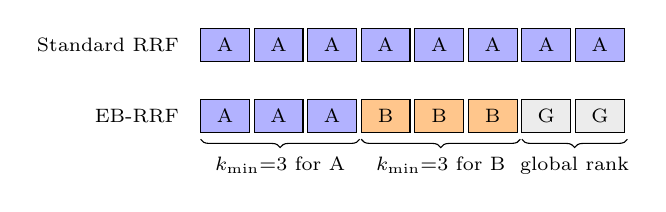
\begin{tikzpicture}[font=\scriptsize, slot/.style={draw, minimum width=0.62cm, minimum height=0.42cm, inner sep=0pt}]
\node[anchor=east] at (-0.15,0.9) {Standard RRF};
\node[anchor=east] at (-0.15,0) {EB-RRF};
\foreach \i in {0,...,7} {\node[slot, fill=blue!30] at (\i*0.68+0.31,0.9) {A};}
\foreach \i in {0,1,2} {\node[slot, fill=blue!30] at (\i*0.68+0.31,0) {A};}
\foreach \i in {3,4,5} {\node[slot, fill=orange!45] at (\i*0.68+0.31,0) {B};}
\foreach \i in {6,7} {\node[slot, fill=gray!15] at (\i*0.68+0.31,0) {G};}
\draw[decorate, decoration={brace, amplitude=3pt, mirror}] (0,-0.3) -- (2.02,-0.3) node[midway, below=3pt] {$k_{\min}{=}3$ for A};
\draw[decorate, decoration={brace, amplitude=3pt, mirror}] (2.04,-0.3) -- (4.06,-0.3) node[midway, below=3pt] {$k_{\min}{=}3$ for B};
\draw[decorate, decoration={brace, amplitude=3pt, mirror}] (4.08,-0.3) -- (5.42,-0.3) node[midway, below=3pt] {global rank};
\end{tikzpicture}
\caption{Illustration of evidence allocation for a two-company query ($K=8$). Standard RRF can give every slot to the more strongly matched company A. EB-RRF first reserves up to three verified slots per company and fills the rest (G) by global rank.}
\label{fig:ebrrf}
\end{figure}

\subsection{Adaptive Hop-Depth Validation}
A query analyser estimates the expected hop depth $h_q$ from lexical and structural cues (e.g., ``indirectly'', ``through its supplier''). A strict gate requires the observed path length $h_{\mathcal{S}}$ to reach $h_q$, which wrongly rejects questions whose relation is stated directly in a filing. The adaptive gate distinguishes the two cases:
\begin{equation}
\mathrm{Hop}(q,\mathcal{S}) =
\begin{cases}
1, & h_{\mathcal{S}} \ge h_q\\
1, & \neg\mathrm{Compound}(q) \wedge \mathrm{DirectValid}(q,\mathcal{S})\\
1, & \mathrm{Compound}(q) \wedge \mathrm{ChainValid}(q,\mathcal{S})\\
0, & \text{otherwise}
\end{cases}
\end{equation}
$\mathrm{DirectValid}$ requires a provenance-verified edge or disclosure connecting the query entities through the requested relation. $\mathrm{ChainValid}$ requires a connected, correctly directed chain for explicitly compound questions such as supplier-risk queries.

\subsection{Regulatory and Jurisdictional Entity Linking}
Filings refer to regulators by full names, abbreviations and jurisdiction-specific phrasing. FinGraph AI links mentions of the Federal Trade Commission, Department of Justice, European Commission, China's State Administration for Market Regulation and the SEC to canonical regulator nodes. This makes regulators usable as query entities and graph seeds. The same component filters references to SEC filing mechanics (e.g., ``filed with the SEC'') so that they are not mistaken for regulatory actions.

\subsection{Temporal and Evidence Validation}
Before generation, each evidence item is checked against \eqref{eq:elig}:
\begin{equation}
\mathrm{Valid}(d_i,t_q) =
\begin{cases}
1, & A_i \le t_q\\
0, & A_i > t_q
\end{cases}
\end{equation}
and ineligible items are removed (Fig.~\ref{fig:temporal}). Graph paths are checked for valid entity connections, and each item must trace to an issuer and accession number. The sufficiency check then verifies that every required entity is covered, that requested relations are present, and that the hop gate is satisfied. If any requirement fails, the system returns a controlled refusal instead of calling the generator.

\begin{figure}[t]
\centering
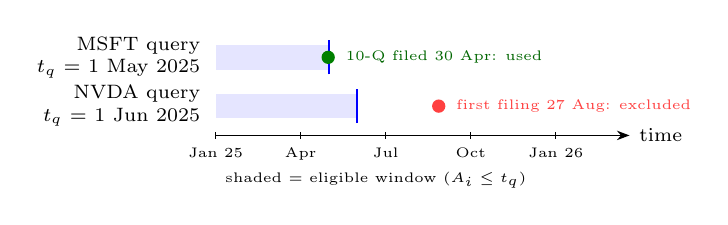
\begin{tikzpicture}[font=\scriptsize, x=0.36cm, y=0.62cm]
% lane labels
\node[anchor=east, align=right] at (-0.2,1.6) {MSFT query\\$t_q$ = 1 May 2025};
\node[anchor=east, align=right] at (-0.2,0.6) {NVDA query\\$t_q$ = 1 Jun 2025};
% eligible windows
\fill[blue!10] (0,1.35) rectangle (4.0,1.85);
\fill[blue!10] (0,0.35) rectangle (5.0,0.85);
\draw[thick, blue] (4.0,1.25) -- (4.0,1.95);
\draw[thick, blue] (5.0,0.25) -- (5.0,0.95);
% filings
\fill[green!50!black] (3.97,1.6) circle (2.4pt);
\node[anchor=west, font=\tiny, text=green!40!black] at (4.25,1.6) {10-Q filed 30 Apr: used};
\fill[red!75] (7.87,0.6) circle (2.4pt);
\node[anchor=west, font=\tiny, text=red!75] at (8.15,0.6) {first filing 27 Aug: excluded};
% axis
\draw[-{Stealth[length=1.6mm]}] (0,0) -- (14.6,0) node[right] {time};
\foreach \x/\l in {0/Jan 25,3/Apr,6/Jul,9/Oct,12/Jan 26} {\draw (\x,0.07) -- (\x,-0.07); \node[below, font=\tiny] at (\x,-0.05) {\l};}
\node[anchor=north west, font=\tiny] at (0,-0.55) {shaded = eligible window ($A_i \le t_q$)};
\end{tikzpicture}
\caption{Point-in-time eligibility on two benchmark queries. A May 2025 query about Microsoft can use the 10-Q filed one day earlier. A June 2025 query about NVIDIA is refused, because the earliest NVIDIA filing in the corpus was not available until August 2025.}
\label{fig:temporal}
\end{figure}

\subsection{Grounded Answer Generation}
Validated evidence is passed to Qwen3.5:4B, run locally through Ollama at temperature 0. The prompt instructs the model to answer only from the supplied evidence, cite evidence identifiers, and emit a fixed refusal string when the evidence does not support an answer. The output is validated a second time: citations must refer to supplied evidence, and cited evidence must satisfy \eqref{eq:elig}. Algorithm~\ref{alg:query} summarises the procedure.

\begin{algorithm}[t]
\caption{FinGraph AI Query Processing}
\label{alg:query}
\begin{algorithmic}[1]
\REQUIRE Query $q$, reference time $t_q$, graph $G$, vector store $\mathcal{V}$
\ENSURE Grounded answer or controlled refusal
\STATE Extract entities $\mathcal{E}_q$, relation intent, hop depth $h_q$, and $t_q$
\STATE Link regulatory and jurisdictional references
\STATE Retrieve semantic candidates from $\mathcal{V}$
\STATE Retrieve graph paths from $G$ by entity-seeded BFS
\STATE Remove candidates with $A_i > t_q$
\STATE Fuse rankings with RRF; if $|\mathcal{E}_q|\ge2$ apply EB-RRF
\STATE Validate provenance, entity coverage and hop gate
\IF{evidence is insufficient}
\RETURN Controlled refusal
\ENDIF
\STATE Generate answer with Qwen3.5:4B ($T=0$)
\STATE Validate citations and their availability times
\RETURN Grounded answer with SEC provenance
\end{algorithmic}
\end{algorithm}

%=====================================================================
\section{Experimental Setup and Results}
%=====================================================================
\subsection{Benchmark and Experimental Environment}
The benchmark was built from the corpus and verified against source chunks and graph edges. Of 65 drafted questions, one was rejected because its comparative evidence was missing from the corpus, leaving 64 verified questions in five categories (Table~\ref{tab:data}). Each answerable question has a reference answer and annotated relevant chunks. Each of the 14 unanswerable questions has a documented reason: a reference date earlier than any eligible filing for the company, a relational link absent from all filings, or a counterfactual premise (e.g., an aircraft-manufacturing claim about Apple). Questions with a reference date test the temporal constraint directly.

All configurations use the same corpus, index, graph, generator and benchmark, so differences in Table~\ref{tab:ablation} reflect configuration changes only. Each configuration was run once with deterministic decoding.

\begin{table}[t]
\caption{Corpus and Benchmark Statistics}
\label{tab:data}
\centering
\footnotesize
\begin{tabular}{lccc}
\toprule
\multicolumn{4}{l}{\textbf{Corpus}}\\
\midrule
SEC filings / companies & \multicolumn{3}{c}{99 / 10}\\
Chunks & \multicolumn{3}{c}{8,181}\\
Graph nodes / edges & \multicolumn{3}{c}{10,054 / 9,822}\\
\midrule
\textbf{Benchmark category} & \textbf{Total} & \textbf{Ans.} & \textbf{Unans.}\\
\midrule
Factual single-hop (FSH) & 13 & 11 & 2\\
Relational single-hop (RSH) & 13 & 11 & 2\\
Temporal point-in-time (TPT) & 13 & 10 & 3\\
Relational multi-hop (RMH) & 13 & 9 & 4\\
Cross-document comparative (CDC) & 12 & 9 & 3\\
\midrule
\textbf{Total} & \textbf{64} & \textbf{50} & \textbf{14}\\
\bottomrule
\end{tabular}
\end{table}

\subsection{Evaluation Metrics}
Each output is classified as an \textit{answer} or a \textit{refusal}. Decision accuracy counts answers to answerable questions and refusals to unanswerable ones:
\begin{equation}
\mathrm{DA} = \frac{N_{\text{ans}|\text{answerable}} + N_{\text{ref}|\text{unanswerable}}}{N_{\text{total}}}\times100.
\end{equation}
The answer rate is the share of answerable questions that received an answer, and the false refusal rate is its complement:
\begin{equation}
\mathrm{FRR} = \frac{N_{\text{false refusals}}}{N_{\text{answerable}}}\times100.
\end{equation}
Refusal recall is the share of unanswerable questions that were refused:
\begin{equation}
\mathrm{RR} = \frac{N_{\text{correct refusals}}}{N_{\text{unanswerable}}}\times100.
\end{equation}
An answer to an unanswerable question is counted as a hallucination. These are decision-level metrics. An ``answer'' is any output that is not a refusal, so they do not by themselves certify that an answer is correct; answer quality is measured separately below.

Answer quality is measured with token-level F1 against the reference answer,
\begin{equation}
F1_{\text{token}} = \frac{2\,P_{\text{token}}R_{\text{token}}}{P_{\text{token}}+R_{\text{token}}},
\end{equation}
and with Exact Match (EM). \textit{Answerable F1} averages over the 50 answerable questions and is the primary quality metric. \textit{Overall F1} averages over all 64 questions and gives a correct refusal a score of 1. It is reported for completeness but is inflated by refusals: $0.3229\cdot\tfrac{50}{64} + \tfrac{14}{64} = 0.4710$.

Temporal reliability is measured by the Future Evidence Infiltration Rate,
\begin{equation}
\mathrm{FEIR} = \frac{N_{\text{evidence with } A_i > t_q}}{N_{\text{evidence}}}\times100,
\end{equation}
computed separately over the retrieved context and the cited evidence.

\subsection{Overall Results}
Table~\ref{tab:overall} reports the full configuration. It reached the correct decision on 59 of 64 questions (92.19\%). It answered 45 of 50 answerable questions, refused all 14 unanswerable ones, and gave no answer to any unanswerable question. FEIR was 0.00\% for both retrieved context and cited evidence. Answer-level overlap remained modest: answerable Token F1 was 0.3229 and EM was 0.02. Mean end-to-end latency was 16.7\,s per question (median 20.4\,s), almost all of it local LLM generation.

\begin{table}[t]
\caption{Overall Results of the Full FinGraph AI Configuration}
\label{tab:overall}
\centering
\footnotesize
\begin{tabular}{lc}
\toprule
\textbf{Metric} & \textbf{Result}\\
\midrule
Decision accuracy & 92.19\% (59/64)\\
Answer rate on answerable questions & 90.00\% (45/50)\\
False refusal rate & 10.00\% (5/50)\\
Refusal recall & 100.00\% (14/14)\\
Answers to unanswerable questions & 0 (0/14)\\
Refusal precision & 73.68\% (14/19)\\
\midrule
Answerable Token F1 & 0.3229\\
Answerable Exact Match & 0.0200\\
Overall Token F1 (refusals scored 1) & 0.4710\\
\midrule
FEIR, retrieved context & 0.00\%\\
FEIR, cited evidence & 0.00\%\\
\midrule
Mean / median latency & 16.7\,s / 20.4\,s\\
\bottomrule
\end{tabular}
\end{table}

\subsection{Ablation Study}
The three components were evaluated individually and together against a base configuration that uses standard RRF, the strict hop gate and standard entity linking (Table~\ref{tab:ablation}). The base configuration reached 85.94\% decision accuracy with nine false refusals. EB-RRF alone and the adaptive hop gate alone each raised the number of answered questions from 41 to 43 (89.06\%), and regulatory linking alone reached 42 (87.50\%). Combining all three gave the best result: 45 answered questions, five false refusals, 92.19\% decision accuracy, and answerable F1 rising from 0.2922 to 0.3229. Refusal recall stayed at 100\% in every configuration, so the whole improvement comes from fewer false refusals and not from a change in abstention on unanswerable questions. Mean latency changed little across configurations (16.3--17.9\,s).

\begin{table*}[t]
\caption{Ablation of FinGraph AI Components on the 64-Question Benchmark}
\label{tab:ablation}
\centering
\footnotesize
\begin{tabular}{lccccccc}
\toprule
\textbf{Configuration} & \textbf{Dec. Acc.} & \textbf{Answered/50} & \textbf{False Ref.} & \textbf{Ref. Recall} & \textbf{Ans. F1} & \textbf{Overall F1} & \textbf{Latency (s)}\\
\midrule
Base (standard RRF, strict hop gate) & 85.94\% & 41 & 9 & 100\% & 0.2922 & 0.4471 & 16.30\\
+ Entity-Balanced RRF only & 89.06\% & 43 & 7 & 100\% & 0.3017 & 0.4544 & 17.95\\
+ Adaptive hop gate only & 89.06\% & 43 & 7 & 100\% & 0.3070 & 0.4586 & 17.02\\
+ Regulatory linking only & 87.50\% & 42 & 8 & 100\% & 0.3029 & 0.4554 & 16.64\\
\textbf{Full FinGraph AI (all three)} & \textbf{92.19\%} & \textbf{45} & \textbf{5} & \textbf{100\%} & \textbf{0.3229} & \textbf{0.4710} & 16.71\\
\bottomrule
\end{tabular}
\end{table*}



\subsection{Per-Category Analysis}
Table~\ref{tab:category} breaks the base and full results down by question category. The full configuration changed four decisions, all from refusal to answer on answerable questions: three relational multi-hop questions and one cross-document comparative question. Factual single-hop, relational single-hop and temporal questions were unchanged. Correct decisions on multi-hop questions rose from 7 to 10 of 13, and answerable F1 in that category nearly doubled (0.1256 to 0.2458). Comparative F1 rose from 0.1816 to 0.2319. This concentration matches the design: EB-RRF targets multi-entity queries and the adaptive gate targets relational ones. Multi-hop and comparative questions are still the weakest categories.

\begin{table}[t]
\caption{Per-Category Correct Decisions and Answerable Token F1 (Base $\rightarrow$ Full)}
\label{tab:category}
\centering
\footnotesize
\begin{tabular}{lcc}
\toprule
\textbf{Category} & \textbf{Correct decisions} & \textbf{Answerable F1}\\
\midrule
FSH (13) & 13 $\rightarrow$ 13 & 0.4173 $\rightarrow$ 0.4173\\
RSH (13) & 12 $\rightarrow$ 12 & 0.3495 $\rightarrow$ 0.3495\\
TPT (13) & 13 $\rightarrow$ 13 & 0.3413 $\rightarrow$ 0.3413\\
RMH (13) & \phantom{1}7 $\rightarrow$ 10 & 0.1256 $\rightarrow$ \textbf{0.2458}\\
CDC (12) & 10 $\rightarrow$ 11 & 0.1816 $\rightarrow$ \textbf{0.2319}\\
\midrule
All (64) & 55 $\rightarrow$ 59 & 0.2922 $\rightarrow$ 0.3229\\
\bottomrule
\end{tabular}
\end{table}



\subsection{Answer Quality Audit and Error Analysis}
Because decision accuracy counts any non-refusal on an answerable question as an answer, the 45 answered outputs were audited post hoc against the cited filing text (Table~\ref{tab:audit}). Thirty-four (75.6\%) were fully supported, with correct entities, figures and reporting periods. For example, the system reported Microsoft's Intelligent Cloud revenue growth of \$12.7 billion (20\%) for the quarter ended 31 March 2025, using only the 10-Q filed the day before the query's reference date. Three answers had a correct core but included an entity introduced by an extraction error, such as an \textsc{acquired} edge created from a strategic-investment disclosure, or a subsidiary recorded as a competitor. Eight were hedged responses stating that the evidence covered only part of the question. The evaluator classifies these as answers because they do not contain the fixed refusal phrase. One of the four questions recovered by the full configuration (a comparative supply-chain question) falls into this hedged group. On the stricter criterion, 34 of 50 answerable questions (68.0\%) received a fully supported answer.

\begin{table}[t]
\caption{Post-Hoc Audit of the 45 Answered Questions (Full Configuration)}
\label{tab:audit}
\centering
\footnotesize
\begin{tabular}{p{5.9cm}c}
\toprule
\textbf{Audit outcome} & \textbf{Count}\\
\midrule
Fully supported by cited SEC evidence & 34 (75.6\%)\\
Correct core, extraction-induced entity error & 3 (6.7\%)\\
Hedged / partial (evidence acknowledged incomplete) & 8 (17.8\%)\\
\midrule
Total answered & 45\\
\bottomrule
\end{tabular}
\end{table}

The five remaining false refusals have two causes. In three cases (an Apple--JPMorgan banking relationship, Alphabet as both competitor and search partner of Apple, and Amazon as a cloud competitor of Microsoft), no filing in the corpus states the required cross-company relation explicitly, so refusal follows from corpus coverage rather than retrieval error. In the other two, the sufficiency gate passed but the generator judged the retrieved passages insufficient for the specific relationship asked about.

\subsection{Qualitative Example}
Fig.~\ref{fig:ui} shows the FinGraph AI interface answering the multi-hop benchmark question RMH-07. The answer names Activision Blizzard and cites two items: the Microsoft 10-K passage describing the acquisition, and the \textsc{acquired} graph edge, each with its availability timestamp. For this query the sufficiency gate reported complete provenance, and the temporal gate reported zero future-dated items (FEIR 0.00\%). The adaptive hop gate accepted the directly stated acquisition relation, so no second hop was required. Under the same interface, the June 2025 NVIDIA query of Fig.~\ref{fig:temporal} returned the fixed refusal string.

\begin{figure}[t]
\centering
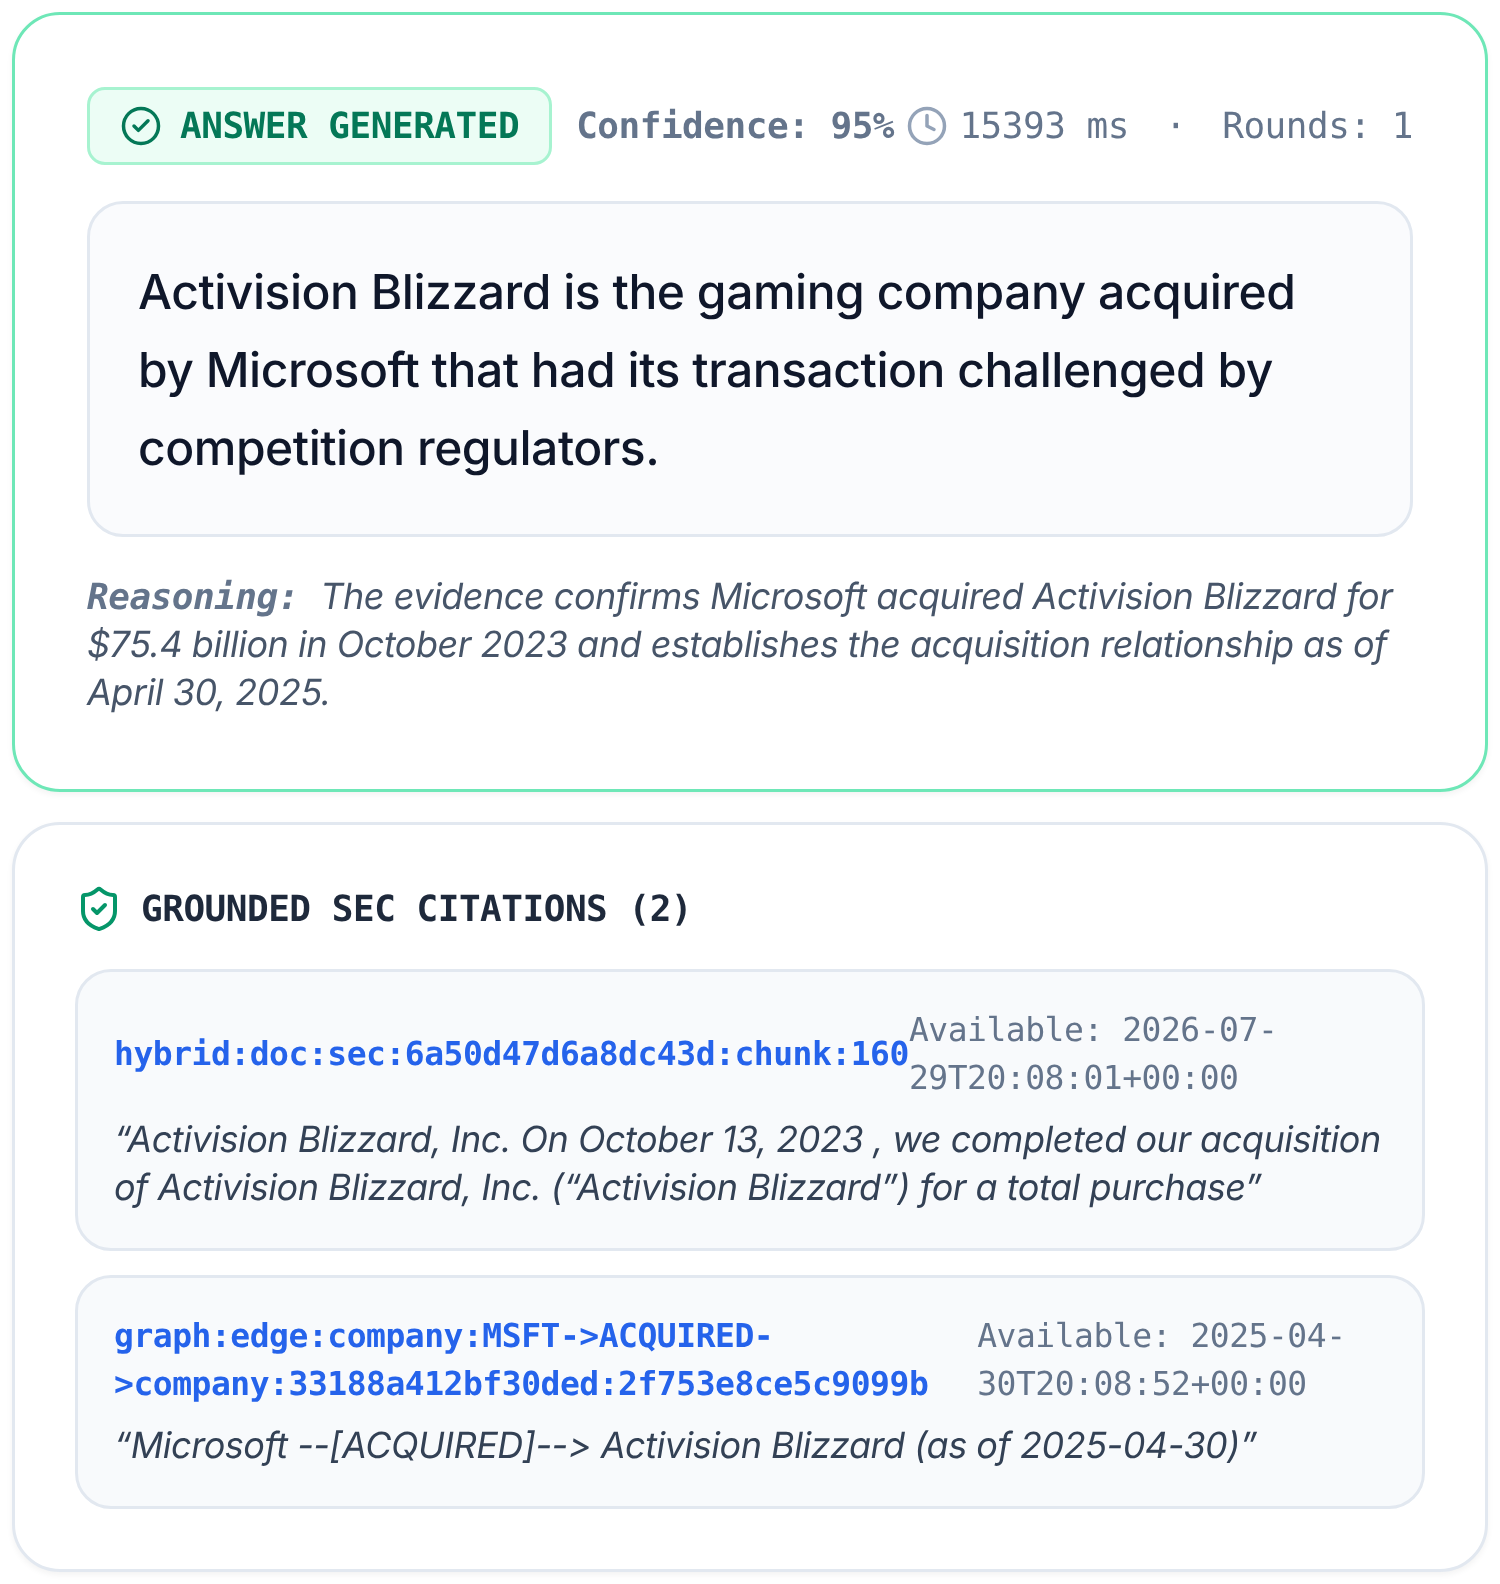
\includegraphics[width=0.96\columnwidth]{ui_rmh07.png}
\caption{FinGraph AI interface output for benchmark question RMH-07 (live run, rendered in the interface's light theme): the generated answer with the model's reasoning and the two grounded SEC citations with their availability times. The interface retrieves 10 evidence items per query rather than the $K=8$ used in the benchmark runs.}
\label{fig:ui}
\end{figure}

\subsection{Discussion}
The results support three observations. First, enforcing availability time at both retrieval and citation removed future-dated evidence entirely on this benchmark (FEIR 0.00\%). Temporal questions were all decided correctly, including refusals where no filing was yet available. Second, the components that broaden evidence (EB-RRF and the adaptive gate) reduced false refusals without weakening abstention: none of the configurations answered an unanswerable question. Third, decision safety and answer completeness are different properties. The audit shows that a correct decision to answer can still yield a hedged or partly incorrect answer, and the low EM reflects that answers are paraphrased rather than copied from the reference.

The two should therefore be reported separately: aggressive answering inflates the answer rate, and aggressive refusal looks safe while being unhelpful.

\subsection{Limitations and Threats to Validity}
\textit{Benchmark size and reuse.} The benchmark has 64 questions from ten large U.S. companies. One question changes decision accuracy by 1.56 points, so differences between single-component configurations should not be over-interpreted. The same benchmark guided the development of the components and was used to evaluate them, and there is no held-out split. The reported figures may therefore be optimistic.

\textit{Missing modality baselines.} Independent vector-only and graph-only baselines have not been completed, so the standalone contribution of each retrieval modality is not measured.

\textit{Evaluation procedure.} Refusals are detected by phrase matching, which counts hedged responses as answers. The audit in Table~\ref{tab:audit} was a single, non-blinded pass. Token F1 and EM capture lexical overlap, not numerical correctness or citation faithfulness.

\textit{Pipeline errors.} Relation extraction introduces some incorrect edges, which can propagate into answers. Results were obtained with one generator (Qwen3.5:4B), and larger models may change the balance between answer quality and abstention.

\textit{Scope of the zero results.} The 0.00\% FEIR and the absence of answers to unanswerable questions apply only to the evaluated queries and do not guarantee the same behaviour on other queries or filings.

%=====================================================================
\section{Conclusion}
%=====================================================================
This paper presented FinGraph AI, a temporal knowledge graph and hybrid GraphRAG framework for multi-hop question answering over SEC filings. It combines structure-aware chunking with availability timestamps, a provenance-linked temporal knowledge graph, hybrid vector and graph retrieval, Entity-Balanced RRF, adaptive hop-depth validation, regulatory entity linking, and an evidence-sufficiency check that permits controlled refusal. On 99 filings from 10 companies and a verified 64-question benchmark, the full framework reached 92.19\% decision accuracy, up from 85.94\% for the base configuration. It refused all 14 unanswerable questions and retrieved or cited no future-dated evidence. The gains came from fewer false refusals on multi-hop and comparative questions, where answerable F1 rose most. Answer quality remains the main open problem: 34 of 50 answerable questions received a fully supported answer, and answerable Token F1 was 0.3229. Future work will add vector-only and graph-only baselines, a larger held-out benchmark across more companies and periods, a semantic refusal classifier, claim-level citation verification, and expert review of financial answers.

\begin{thebibliography}{00}
\bibitem{ertugrul2026rag} M. A. C. Ertu\u{g}rul, A. N. Acar, and Z. H. Kilimci, ``RAG-powered financial trend analysis system using Borsa Istanbul indices,'' in \textit{Proc. 34th Signal Processing and Communications Applications Conference (SIU)}, 2026, doi: 10.1109/SIU71813.2026.11636643.
\bibitem{yahathugoda2026kgatfin} Y. R. Yahathugoda, T. Osman, and J. Bird, ``KGATFin: Knowledge graph augmented transformers for financial analytics,'' in \textit{Proc. 8th International Conference on Pattern Analysis and Intelligent Systems (PAIS)}, 2026, doi: 10.1109/PAIS69842.2026.11605323.
\bibitem{yarlagadda2026kg} K. C. Yarlagadda, ``Knowledge graph enhanced transformer framework for semantic product search and financial document analysis,'' in \textit{Proc. IEEE Conference on Computer Applications (ICCA)}, 2026, doi: 10.1109/ICCA69280.2026.11485785.
\bibitem{jain2025dynamic} Y. K. Jain, R. Bajaj, A. Khare, P. Beriwala, A. Pandey, and M. S. Bhokare, ``Dynamic knowledge graphs for predictive business insights: A fusion of NLP and graph neural networks,'' in \textit{Proc. International Conference on Automation and Computation (AUTOCOM)}, 2025, doi: 10.1109/AUTOCOM64127.2025.10956693.
\bibitem{chai2026graphllm} Z. Chai, T. Zhang, L. Wu, K. Han, X. Hu, X. Huang, and Y. Yang, ``GraphLLM: Boosting graph reasoning ability of large language model,'' \textit{IEEE Transactions on Big Data}, vol. 12, no. 2, 2026, doi: 10.1109/TBDATA.2025.3627488.
\bibitem{van2026llmstock} N. L. Van, V. T. Hoang, N. Dinh, H. N. Quoc, K. Tran-Trung, and T. T. Cong, ``LLM-based stock price and volatility prediction: A multi-modal deep learning framework integrating financial news sentiment and technical indicators,'' in \textit{Proc. 2nd International Conference on Computational Intelligence Approaches and Applications (ICCIAA)}, 2026, doi: 10.1109/ICCIAA68481.2026.11544016.
\bibitem{yang2025timerag} S. Yang, D. Wang, H. Zheng, and R. Jin, ``TimeRAG: Retrieval-augmented generation for time-series forecasting,'' in \textit{Proc. IEEE International Conference on Acoustics, Speech and Signal Processing (ICASSP)}, 2025, doi: 10.1109/ICASSP49660.2025.10889933.
\bibitem{icocics2025earnings} ``A multi-model approach to sentiment analysis of earning calls: Integrating Whisper, BART, and FinGPT,'' in \textit{Proc. IEEE 2nd International Conference on Cryptography, Informatics, and Cybersecurity (ICoCICs)}, 2025, doi: 10.1109/ICoCICs68032.2025.11384062.
\bibitem{sabuncuoglu2025bias} A. Sabuncuoglu and C. Maple, ``Identifying representation bias in large language models used in financial sentiment analysis,'' in \textit{Proc. IEEE Symposium on Computational Intelligence for Financial Engineering and Economics (CIFEr)}, 2025, pp. 1--7, doi: 10.1109/CIFER64978.2025.10975731.
\bibitem{kamlakshya2025agentic} T. Kamlakshya, ``Agentic RAG systems for real-time financial decision making: A multi-agent framework with model context protocol integration,'' in \textit{Proc. IEEE International Conference on Information Technology, Electronics and Intelligent Communication Systems (ICITEICS)}, 2025, doi: 10.1109/ICITEICS64870.2025.11341179.
\end{thebibliography}

\end{document}
